\documentclass[letterpaper]{article}
\usepackage[T1]{fontenc}
\usepackage[colorlinks]{hyperref}
\usepackage[pdftex]{graphicx}

\newcommand{\cpp}{C{\nobreak +}{\nobreak +}}
\newcommand{\code}[1]{#1}
\renewcommand\_{\textunderscore\allowbreak}


\title{Genetic Chess}
\author{Mark Harrison}

\begin{document}

\maketitle

\begin{abstract}
This work is a program for evolving chess-playing AIs.  By pitting a population of AIs against each other in chess matches, killing off the losers, and breeding the winners, it is hoped that one specimen will be able to stand up against a more traditionally developed engine (if only on the easiest difficulty setting). Though it is written in \cpp{}, it is the hope of the author that the style and architecture are comprehensible.
\end{abstract}

\tableofcontents{}


\section{Building}
Though there is nothing OS-specific about the \cpp{} code, the Makefile is written for a Linux system. The code can be compiled with any \cpp{} compiler via
\begin{quote}
	\code{<compiler> -I include <all *.cpp files>}
\end{quote}
where \code{-I} indicates the option to specify the base directory of the header files.

\subsection{Linux}
Run \code{make} to create release and debug executables in a \code{bin/} subfolder that will be created if it does not already exist. If, in the course of working on this project, new files are created or the \code{\#include} files are changed within a file, run \code{python create\_Makefile.py} to regenerate the Makefile. This python script assumes all \code{*.cpp} and \code{*.h} files in the current directory and all subfolders are part of the project and need compiling.


\section{Running}
\label{running}
\begin{description}
	\item[\code{genetic\_chess -genepool [file\_name]}]
This will start up a gene pool with Genetic\_AIs playing against each other--mating, killing, mutating--all that good Darwinian stuff. The required file name parameter will cause the program to load a gene pool and other settings from a configuration file. A record of every genome and game played will be written to text files.

	\item[\code{genetic\_chess <-player> <-player>}] Starts a local game played in the terminal with an ASCII art board. The first parameter is the white player, the second is black. The \code{<-player>} argument is replaced with one of the following:
	\begin{description}
		\item[\code{-human}:] a human player entering moves on the command line and seeing the results on a text-based drawing of the board. Moves are specified in standard algebraic notation (SAN) or in coordinates that indicate the starting and ending square. 
		\item[\code{-genetic}:] a Genetic AI player. If a file name follows, load the genes from that file. If there are several genomes in a file, the file name can be followed by a number to load the genome with that ID. If no number is specified, then there are two possibilities:
		\begin{itemize}
			\item If the genome file is the output of a gene pool run, then the AI with the smallest ID that was still alive is chosen. As the oldest surviving AI, it is the nearly the most evolved while still having been tested.
			\item Otherwise, the last genome in the file is loaded (presumably this one is the most evolved). If there is another file containing records of games played during a gene pool run that has the same name as the genome file name with an extra suffix ``\_games.txt'', then the last genome with at least 3 wins will be selected.
		\end{itemize}
		\item[\code{-random}:] an AI player that chooses a random legal move at each turn.
	\end{description}
\end{description}
Genetic Chess can communicate with GUI chess programs through the \href{https://www.gnu.org/software/xboard/engine-intf.html}{Chess Engine Communication Protocol}, including xboard, PyChess, Cute Chess, and others. When using Genetic Chess this way, only specify the arguments for a single player (\code{-genetic} or \code{-random}). The program will then wait for communication from the GUI.


\section{Non-Evolutionary Aspects}

These sections describe the aspects of the chess AI that are not genetically modifiable, usually because of at least one of the following reasons:
\begin{itemize}
	\item There is no sense in which the aspect of play is improvable. Any modification would be detrimental to the chess playing;
	\item It would take far too much time to evolve that aspect of play from a random starting configuration, or it would interfere too much with the evolution of other aspects;
	\item I cannot conceive of how to represent the state space of that particular play strategy so that it may be genetically encoded.
\end{itemize}
On the last point, it has been suggested to me that, instead of the specific genes listed in Section~\ref{gene-section}, the genes should encode more abstract and generic strategies and heuristics for evaluating a board state. While this would probably better mimic biological evolution (wherein adenine and thymine are rather neutral as to their teleology), I have no idea how to program such an abstract representation and how to translate the action of such genes into chess moves. So, what results from all this programming is a glorified tuning algorithm for parameters in predefined genes with hard-coded meanings.

On the other hand, so is every other genetic algorithm (see \cite{evolved-antenna}, \cite{evolved-stellarator}, and others). Plus, these genes can be deactivated through mutation, so these AIs are perfectly capable of telling me exactly what they think of my painstakingly crafted genes.\footnote{The little ingrates!}

\subsection{Endgame Scoring}

Winning gives an infinite score.
Losing gives a negative infinite score.
Draw gives zero.

Why not evolve these numbers? While the priorities of various genes can be varied to yield different playing styles, the only reasonable score to assign to a win is one that is larger than any other score. It can only be a disadvantage to prefer anything to a winning move. While this would result in upward evolutionary pressure on the score assigned to winning, it would stall the evolution of all other genes while the score assigned to winning was pushed high enough to always be preferred.

The specific values were chosen to make the scoring symmetrical between the two players, in that the score for one side is the negative of the score as seen from the other side (assuming the same player does the scoring). What is good for one player is bad for the other player by the same amount.

\subsection{Mini-maxing}

The principle behind the minimax algorithm is that the quality of a move is measured by the quality of moves it allows the opponent to make. Of course, the quality of those moves is measured by the quality of the moves that follow. Ideally, the only required board evaluation scores would be \(1\)~for a win, \(0\)~for a draw, and \(-1\)~for a loss, and all possible sequences of moves would be examined to find the guaranteed outcome. Unfortunately, the number of positions to examine in a typical game is far too large to examine in a few minutes, so the search has to be cut off at some point and a heuristic evaluation employed to estimate the probability of winning from that stopping point. In this program, the decision of when to stop and the heuristic evaluation is genetically determined and evolved over many generations.

\subsection{Alpha-Beta Pruning}

Alpha-beta pruning is based upon keeping a record of two game state evaluations:
\begin{description}
	\item[Alpha:] is the highest score that the player whose turn it is guaranteed once the game reaches the current state and cannot be avoided by the opponent making different moves later in the game. That is, the player whose turn it is at this point in the game tree can force the game into a state with at least this score.
	\item[Beta:] is the lowest score to which the opponent can limit the current player by making different moves earlier in the game. If the current player finds a move with a higher score than Beta, then the opponent would make an earlier move that makes this game state impossible to reach. This is called ``refuting'' the move. Once such a move is found, the examination of moves from the current game state is abandoned, as the opponent will not allow this state to be reached.
\end{description}
Each time a move examination reaches a greater depth in the game tree, these values switch roles to represent the view of the board from the opponent's perspective.

An extra optimization implemented in this program is one where the search is cut off if Alpha represents a win at a shallower depth in another branch of the tree branch. If a checkmate can be forced in fewer moves by making different earlier moves, there's no point in looking for a win in the current move sequence.

\subsection{Principal Variation Recall}

If the best move is chosen based upon the probable resulting future board state based on a sequence of moves (a variation) found through minimaxing with alpha-beta pruning, and if the opponent makes the next predicted move in that variation, then the moves leading to that board state are examined first during the next move. This high-scoring board state should lead to early cutoffs from alpha-beta pruning, especially if that board state was a game-ending state. If that board state is actually avoidable by the opponent, then the shallower depth of that state during the next turn should lead to a faster refutation, leaving time to examine alternate variations.


\section{The Genome}
\label{gene-section}
The genome is the repository for genetic information in the Genetic AIs and controls all aspects of game play not mentioned in the previous section. All are subject to mutation, which can change the behavior and influence of a given gene, or even deactivate it entirely. Gene deactivation is a strategy for exiting local peaks in fitness since a gene can still mutate when deactivated. Since it feels no evolutionary pressure, the deactivated gene is free to random walk somewhere else, perhaps to a more advantageous state that will be discovered upon reactivation.

\subsection{Regulatory Genes}
A regulator gene refers to a gene that does not participate in evaluating the state of a game board. These genes either control other aspects of the Genetic AIs or are queried by other genes for information.

\subsubsection{Piece Strength Gene}
This gene specifies the importance or strength of each different type of chess piece. Other genes like the Total Force Gene (Section~\ref{total-force}) reference this one for their own evaluation purposes.

The number associated with each piece is not scaled to any other piece, but before a piece strength is returned, it is scaled so that that total value of all the pieces at the start of the game (8~pawns, 2~rooks, 2~knights, 2~bishops, and 1~queen) equals~1. This prevents mutations in this gene from changing the priorities of other genes that reference this one. In other words, if a series of mutations doubles the strength of all pieces, the Total Force Gene will not subsequently return double the score for the same board state. Only mutations that change piece strengths with respect to other pieces are effective. The king is not assigned a strength because it is always on the board, so it cannot affect the move chosen.

\subsubsection{Look Ahead Gene}
This gene determines all aspects of the Genetic AIs time management. There are four genetically determined components to this gene that determine how the AI spends its time:
\begin{enumerate}
	\item the average number of moves per game,
	\item the minimum number of moves to leave time for (or, the maximum fraction of time to use),
	\item the number of positions that can be examined per second,
	\item a constant related to probabilistically looking further ahead when no enough time is allocated.
\end{enumerate}
When it starts the algorithm to choose a move, it allocates a fraction of the time left on the clock so that all subsequent moves get equal time. That is, if there are 20~moves estimated to be left in the game, then \(1/20\)~of the remaining time is used for this move. The number of moves left is estimated by assuming the number of moves in a game is modeled by a Poisson distribution with a mean given by the first parameter listed above:
\[N = \frac{\sum_{i = n + 1}^\infty P(i)\times{}i}{\sum_{i = n + 1}^\infty P(i)} = \frac{\sum_{i = n + 1}^\infty \frac{N_g^{\phantom{g}i}}{i!}\times{}i}{\sum_{i = n + 1}^\infty \frac{N_g^{\phantom{g}i}}{i!}}\]
where \(N\) is the estimated total number of moves in the game, given that \(n\) moves have already ben made, \(N_g\) is the genetically determined average moves per game (the first parameter in the list above). The Poisson probability distribution is given by
\[P(i) = e^{-N_g}\frac{N_g^{\phantom{g}i}}{i!}.\]
Despite the summation going to infinity, the computation does halt because the probability drops off exponentially for \(i > N_g\) and the summands fall below floating point resolution

Unfortunately, it turns out that the Poisson distribution is not a good fit for the lengths of games. As can be seen in Figure~\ref{game-length-plot}, a truncated normal distribution is a better fit, although the real distribution has a fatter right tail and is near zero for zero-move games.
\begin{figure}[tbh]
	\centering
	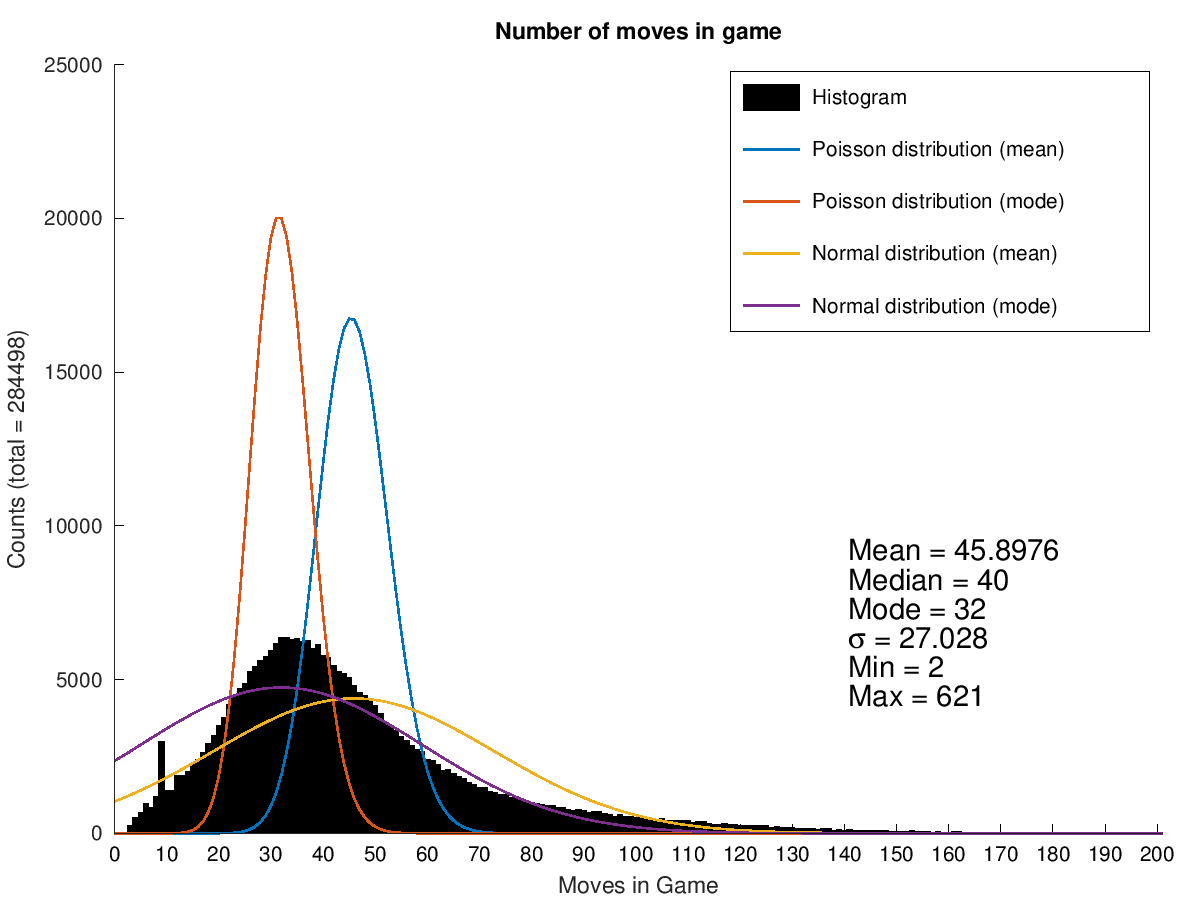
\includegraphics[width=\textwidth]{game_length_distribution.png}
	\caption{The distribution of the number of moves in a game (with one move consisting of both a black and white play). The (mean) and (mode) designations in the legend indicate which statistic was used as the mean parameter of the distribution. The spike at 9~moves was created just after a change to the program that resulted in much faster changes in board state (see Section~\ref{board-submit-move-section} for details).}
	\label{game-length-plot}
\end{figure}

Further research has shown that the log-normal distribution~\cite{log-norm-wiki} is a much better fit to the data, as pointed out on Stack Exchange~\cite{log-norm-chess-se}. The probability of a game taking $i$ moves to complete is given by
\[P(i) = \frac{1}{iS\sqrt{2\pi}} e^{-\frac{1}{2}\left(\frac{\ln{i} - M}{S}\right)},\]
where \(S\) and \(M\) are the standard deviation and mean of \(\ln{N}\), respectively. A plot of the number of moves in a long gene pool run can be seen in Figure~\ref{log-norm-plot}. This probability function can be directly substituted into the above equation for the number of moves left. The other advantage of this distribution is that the expected number of moves has an analytic solution (when the \(\textrm{erf}()\) function is included).
\begin{figure}[tbh]
	\centering
	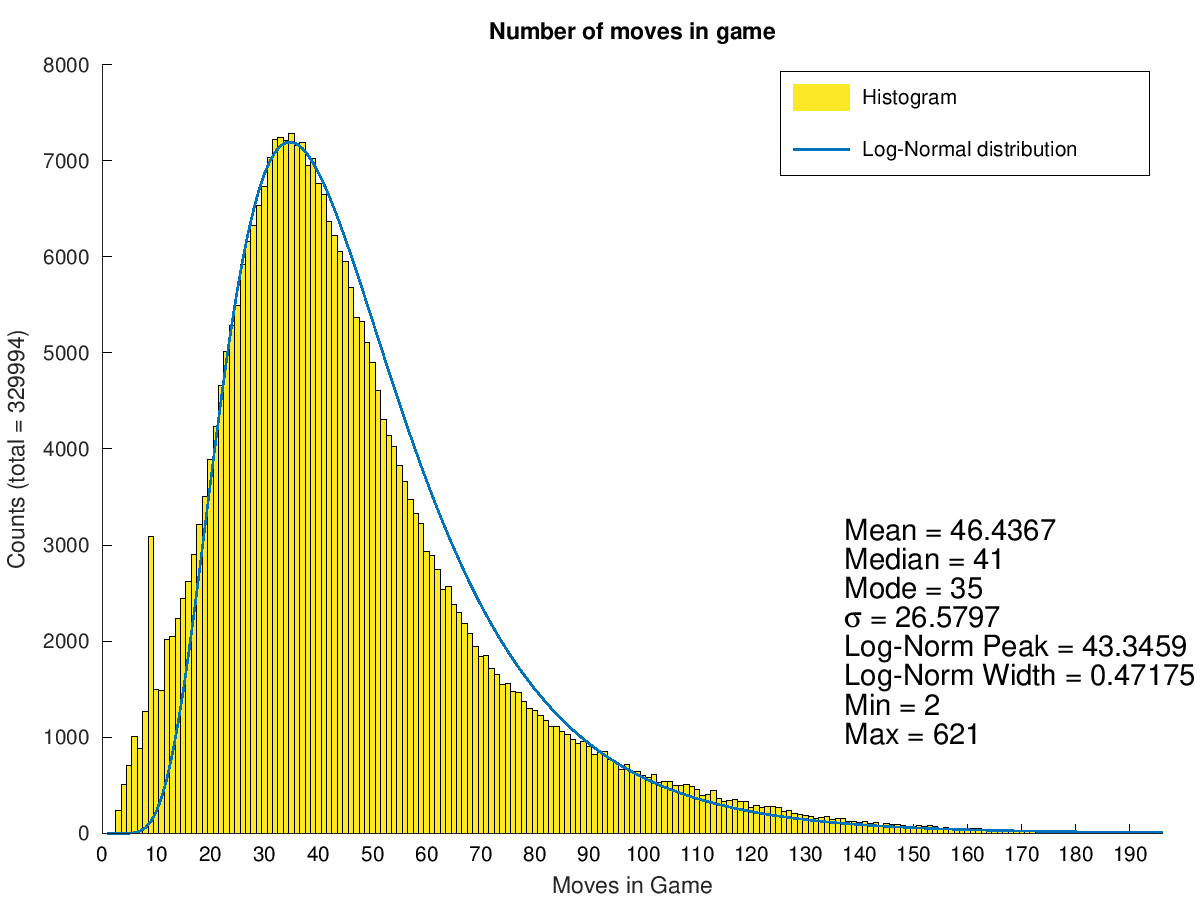
\includegraphics[width=\textwidth]{game_length_log_norm_distribution.png}
	\caption{The distribution of the number of moves in a game with a log-normal fit. The Log-Norm parameters listed are \(M\) for the Peak parameter and \(S\) for the Width parameter. To obtain a better fit, only games longer than 15~moves were considered, as shorter games were primarily by ill-adapted AIs, especially at the beginning of the gene pool run.}
	\label{log-norm-plot}
\end{figure}

If the expected number of moves left is less than the minimum number of moves to allocate time for (the second parameter in the above list), then that minimum is used instead. Finally, if the result of that comparison is greater than the number of moves that will result in a clock reset, then the latter will be used to determine how much time will be used. In a game with 40/5~time control, where five minutes are added to the clock every 40~moves, the 40th move can use all the remaining time since an extra five minutes will be added after the move. Whatever the final number of moves left in the game is determined to be, the time on the clock is divided by that number to determine how much time to take to choose a move.

When choosing a move from the current board, the amount of time to consider a move is equal to the amount of time left for this board position divided by the number of legal moves left to consider. This naturally limits the depth of search while allowing deeper searches for positions with fewer legal moves. If a move examination is cut off early for whatever reason (e.g., a game-ending move is found or through alpha-beta pruning), then the remaining time for that move is available for as yet unexamined moves.

An effective chess player needs to look at the consequences of a move to decide if a move is good. In order to decide how far to look ahead (and if there is time remaining to examine this move), the AI divides the number of legal moves in the board position after the move under consideration by the number of positions it can examine per second (the third parameter in the list above). This is the time it requires to examine the resultant position. If this is less than the time allocated for the move, the algorithm looks ahead (the function recurses) to examine the moves the opponent can make in response. Otherwise, the AI looks ahead with a probability given by
\[P(t, T; k) = \left(\frac{t}{T}\right)^\frac{1-k}{k}\]
where \(t\) is the time available for a move, \(T\) is the time needed to look ahead, and \(k\) is a genetically determined constant and the fourth parameter in the list above. The parameter \(k\) varies between 0~and~1, resulting in an exponent that varies from \(\infty\) and \(0\), respectively. When \(k=0.5\), the exponent is equal to one, and the probability of look ahead is proportional to the time remaining. If \(k < 0.5\), then the exponent is less than one, resulting in higher probabilities since \(x^p > x\) for \(0 < x < 1\) and \(p < 1\).  If \(k > 0.5\), then the exponent is greater than one, resulting in lower probabilities. Plus, transforming \(k \to 1-k\) transforms the exponent into its inverse, giving a nice symmetry to the parameter in that \(k\) and \(1-k\) are aggressive-conservative mirror images.

\subsubsection{Branch Pruning Gene (deleted)}

This gene would prevent the game tree search from examining the moves following a certain move if the board state that immediately resulted from that move was of a sufficiently lower score than the present board state. This gene was supposed to save time by skipping in-depth examinations of moves that were obviously immediately bad. This gene was deleted because it seemed to slow down the evolution of other genes by harshly punishing large swings in board value. This would cause genes that increased in priority to trip this gene, preventing look-ahead, and thus good play.

\subsection{Board-Scoring Genes}
These genes are used to give a score to a board state. The higher the score, the more desirable the moves that lead to this board. The score is calculated by
\[Score = \sum_g Priority(g) \times Score(g,B)\]
where \(g\) represents each gene, \(Priority(g)\) is a genetically determined scalar multiplicative factor that determines how much the gene's score of the board influences the final score, and \(Score(g,B)\) is the result of the scoring procedure of that gene on a given board \(B\). In general, the scores are scaled so that a typical board state gets a score of 1 from any gene. For example, the Freedom to Move Gene divides the number of legal moves by the number of legal moves at the start of the game (20 for standard chess). The Total Force Gene returns 1 for the pieces at the start of the game, so promoting a pawn can result in a score of more than one.

Since it is not only important to find position that are advantageous to the player, but also disadvantageous to the opponent, the final heuristic score for a board position is
\[Heuristic\ Score = Score(Player) - Score(Opponent).\]

\subsubsection{Total Force Gene}
\label{total-force}
This gene sums the strength (according to the Piece Strength Gene) of all the player's pieces on the board.

A unique aspect of this gene is that it is the only one whose priority is constrained to be non-negative. This was done to avoid a genome where the Total Force Gene and the Opponent Pieces Targeted Gene have oppositely signed priorities. This would cause mixed pressure on the Piece Strength Gene values, interfering with its evolution. This does not limit the expressiveness of this gene, since the Piece Strength Gene and the Opponent Pieces Targeted Gene are free to take on negative values. Any genome with a negative priority on the Total Force Gene is equivalent to another genome with the signs of the three mentioned genes' priorities negated.

\subsubsection{Freedom to Move Gene}
This gene counts the number of legal moves available in the current position.

\subsubsection{Pawn Advancement Gene}
This gene measures the progress of all pawns towards the opposite side of the board. Extra points are awarded to board states that have pawn promotions as past moves in order to prevent promotions from being penalized when such moves remove pawns from the board.

\subsubsection{Opponent Pieces Targeted Gene}
This gene sums the total strength (as determined by the Piece Strength Gene) of the opponent's pieces currently under attack.

\subsubsection{Sphere of Influence Gene}
This gene counts the number of squares attacked by all pieces. Bonus points are awarded if the square can be attacked with a legal move. That is, if a piece cannot reach a square in one move (perhaps because such a move is blocked by another piece), then that square is still counted as falling under the influence of the side owning that piece. Further bonus points are awarded based on how close the attacked square is to the king.

\subsubsection{King Confinement Gene}
This gene counts the squares the king can reach given unlimited legal moves. Squares that take a larger number of moves to reach are given lower scores. Kings that are hemmed in by squares occupied by friendly pieces and squares attacked by the opponent result in a low score from this gene. This is a measure of how much room the king has to maneuver and escape. It is somewhat in opposition to the King Protection Gene.

\subsubsection{King Protection Gene}
This gene counts the squares that have access to the king by any valid piece movement and are unguarded by that king's other pieces. In other words, it measures how exposed the king is to hypothetical attacks. A higher score means a less exposed king.

\subsubsection{Castling Possible Gene}
This gene returns a positive score to indicate that castling is possible or has already happened. A higher score indicates that castling is closer to being a legal move due to intervening pieces being moved away. The score can vary based on a genetically determined preference for kingside or queenside castling.




\section{The Gene Pool: On the Care and Feeding of Chess AIs}

In each generation, the players in a gene pool are randomly matched up with each other to play a single game of chess. If the game ends with a winner, whether through checkmate or time violation, then the two players mate to produce an offspring by picking each gene randomly from either parent with equal probability. The offspring is then subject to a a single extra mutation procedure wherein two genes on average are individually mutated. Finally, the offspring replaces the loser in the gene pool. This way, some the genes of losing players are passed on and only slowly weeded out since a single game does not actually provide much information about the fitness of any gene with respect to game play.

If the game ends in  a draw, then one of two things happens. With high probability--currently 95\%--the players are left as they are and will participate in the next generation. The other possibility is that one of the players is randomly picked to mate with either a randomly generated AI, or a randomly chosen past AI, even long dead ones. The chosen player is then replaced by the offspring. This happens with low probability because it destroys genetic information. By ``information,'' I mean filtered genomes. If a gene (including small variations, given the continuous nature of these genotypes) is present is a large percentage of the species, then that gene must have been present in a great number of AIs that were victorious in their games through many generations and many different opponents. Genes found in losing organisms slowly fade away as their host organisms fail to reproduce. However, it is necessary to keep a pool from stagnating due to never-ending drawn games. Bringing in a randomly generated AI injects new genetic information into the pool (though with low probability of high-quality information). Bringing back dead AIs injects good information from the past and should help to keep a gene pool from becoming trapped in a self-reinforcing, pathological playing style that only works against similar players. In effect, both of these strategies are meant to kick a gene pool off of a local peak of genetic fitness.

One final means of preventing gene pool stagnation and preserving genetic diversity is the use of multiple gene pools. Each gene pool evolves separately for a long time, allowing each to genetically diverge. Then, every once in a long while (the time being user-specified), the best player from each pool is transferred to the next pool over. Thus, the best genes are further spread afield so that they can be tested against a wide range of opponents. A useful measure of a pool's strength is how long its best player survives when it enters a new pool.

\subsection{Gene Pool Configuration File}
A gene pool is configured with a text file that is reference in the program starting arguments (see Section~\ref{running}). An example gene pool configuration file is presented below.
\begin{verbatim}
# Gene Pool Configuration (# indicate comments)

# The number of processors used will be the minimum
# of this number and half the gene pool population.
maximum simultaneous games = 8

# How many players in each pool
gene pool population = 16

# How many gene pools
gene pool count = 3

# Probability of killing a player after a draw
draw kill probability = 0.05

# Games in between swapping players between pools
pool swap interval = 1000

# Oscillating game time
#
# The time for each game starts at the minimum, then goes up
# by the increment after each round of games. When it reaches
# the maximum, the increment is reversed and the time for each
# game goes down until it reaches the minimum. Then, the cycle
# starts again.
minimum game time = 30 # seconds
maximum game time = 120 # seconds
game time increment = 0 # seconds

# The name of the file where the genomes will be recorded.
# Games will be recorded in a file with "_games.txt" appended
# to the name.
gene pool file = pool.txt
\end{verbatim}

\subsection{Gene Pool Output}
An example of typical output during a gene pool run is shown below:
\begin{verbatim}
Gene pool ID: 0  Gene pool size: 16  New blood introduced: 126 (*)
Games: 22024  White wins: 10469  Black wins: 9562  Draws: 2737
Time: 38.538 sec   Gene pool file name: pool.txt
    ID   Wins  Streak  Draws  Streak
 59014      9       7      1       0 T
 59031      3       3      0       0
 59054      1       0      2       2
 59055      2       2      0       0
 59074      1       1      0       0
 59077      1       1      0       0
 59078      1       1      0       0
 59081      1       1      0       0
 59095      0       0      0       0
 59096      0       0      0       0
 59097      0       0      0       0
 59098      0       0      0       0
 59099      0       0      0       0
 59100      0       0      0       0 *
 59101      0       0      0       0
 59102      0       0      0       0

59055 vs 59097: White!
59074 vs 59101: Black!
59102 vs 59100: White!
59096 vs 59014: None! 59014 mates with random / 59096 dies
59031 vs 59078: None!
59054 vs 59095: Black!
59098 vs 59099: Black!
59081 vs 59077: White!

Most wins:     18 by ID 20968
Longest lived: 27 by ID 45394
\end{verbatim}
The \verb|Streak| column indicates the current number of consecutive wins or draws a player has attained in the last few games. In the example above, Player 59014 is on a seven-game winning streak following its last draw. Player 59054 has drawn its last two games.

The asterisk (\verb|*|) indicates an offspring of the result of a drawn match. Note that the outcome of the game between 59096 and 59014 means that another such offspring will be brought into this pool for the next round. The (\verb|T|) indicates that it is the best AI from another gene pool that has been copied to this pool.


\section{Some Consistent Results (in rough order of discovery)}

Here are a few results that are reliably reproduced in multiple simulations. In these runs, there were three gene pools with 16~players each (so the number of games equaled the number of processors on my computer, i.e.,~8). Each game is played with 30~seconds per side for the entire game with no increment.

\subsection{Piece values are rated in near-standard order.}
In descending order of valuation by a Genetic\_AI: Queen, Rook, Bishop and Knight nearly equally, and Pawn. As time goes on,there is a lot of variation, especially in the relative order of the Rook, Knight, and Bishop. But, the standard order is preserved for the most part, as can be seen in Figure~\ref{piece-value-plot}.
\begin{figure}[htb]
	\centering
	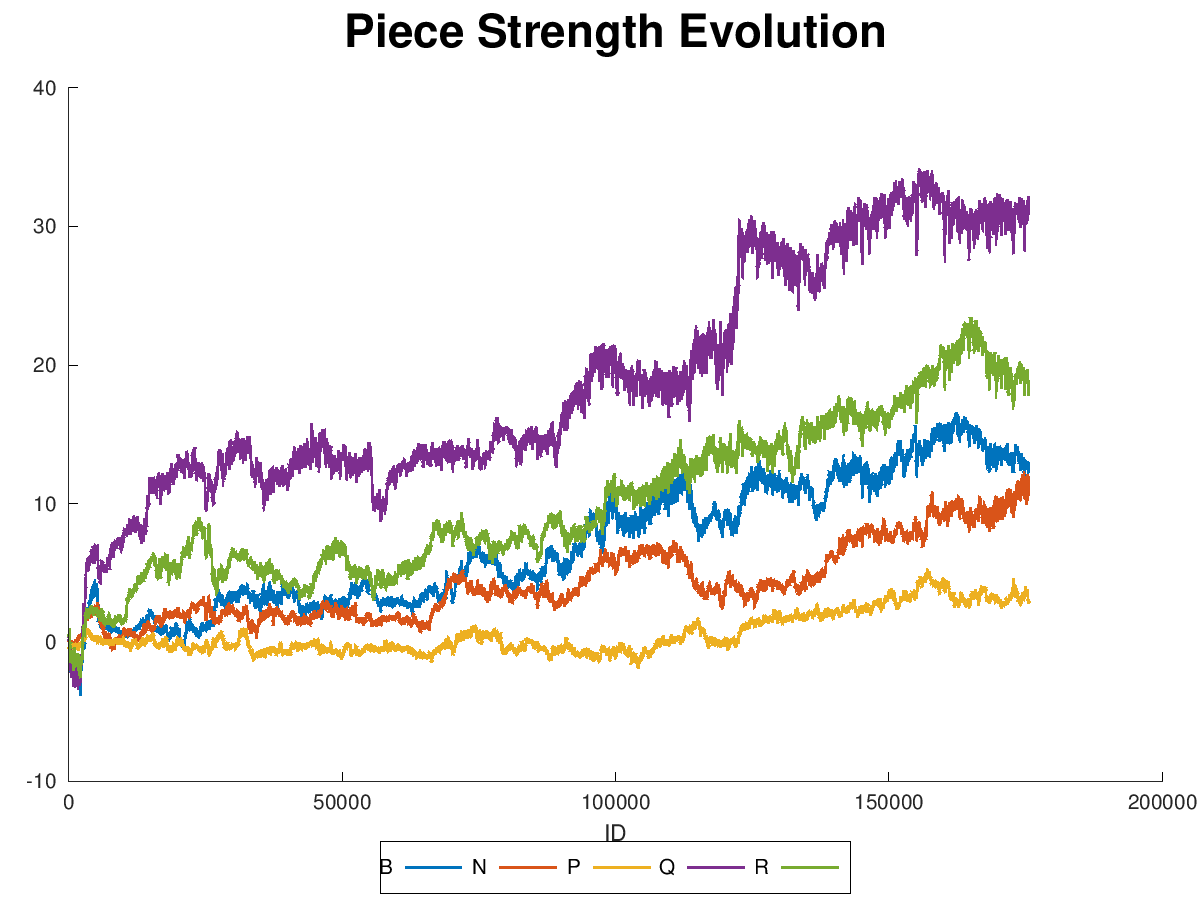
\includegraphics[width=\textwidth]{pawn-crash-strength-plot}
	\caption{The evolution of the value of pieces to the AIs. The small bump near ID~\#120,000 in the strength of a pawn that caused the Pawn Advancement Gene crash seen in Figure~\ref{pawn-crash}}
	\label{piece-value-plot}
\end{figure}

\subsection{White has an advantage.}

Of the games ending in checkmate, white wins about 10\% more often than black. Figure~\ref{win-lose-plot} shows that the advantage is persistent through almost the whole of a long gene pool run. Wins by time are shared by black and white equally (see Figure~\ref{game-ending-plot}).
\begin{figure}[htb]
	\centering
	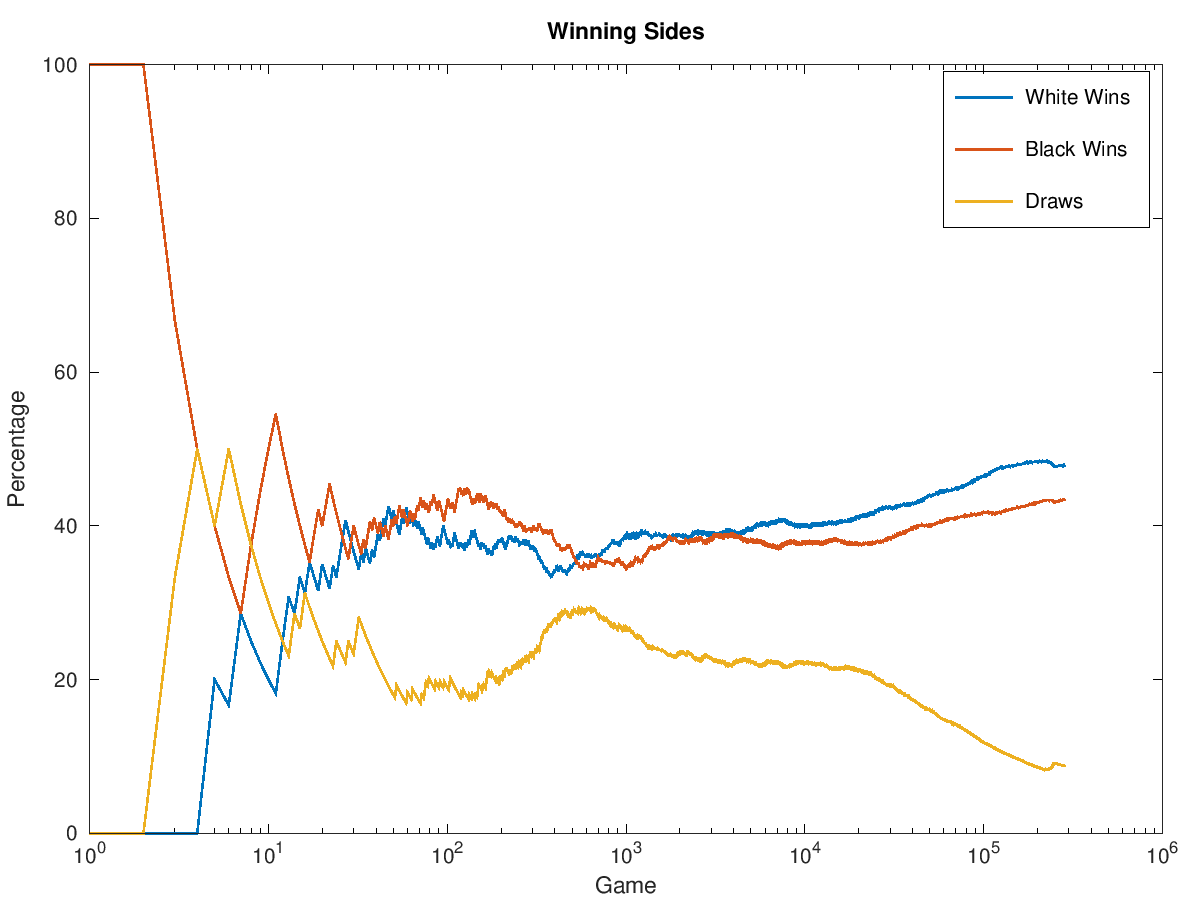
\includegraphics[width=\textwidth]{win-lose-plot}
	\caption{The percentage of games won by white, black, or neither over the course of a gene pool run. The advantage that white has over black seems persistent. Also, as the AIs evolve, the rate of draws decreases, presumably because they evolve a genome that can tell the difference between a good and bad position.}
	\label{win-lose-plot}
\end{figure}

\subsection{The Total Force Gene and the Pawn Advancement Gene typically dominate.}

The Pawn Advancement Gene usually gains higher priority first, probably because it is the simplest gene that makes an immediate difference in the game. Push the pawns forward both threatens the opponent's pieces with low-risk attacks and increases the chances of promotion.

\subsubsection{Late-Breaking News: The Pawn Advancement Gene is a temporary substitute for a valid value of the pawn in the Piece Strength Gene.}

Near the birth of the Genetic AI with ID~\#120,000, the Pawn Advancement Gene suddenly died off, with nearly all AIs in the gene pool deactivating the gene simultaneously (see Figure~\ref{pawn-crash}).
\begin{figure}[htb]
	\centering
	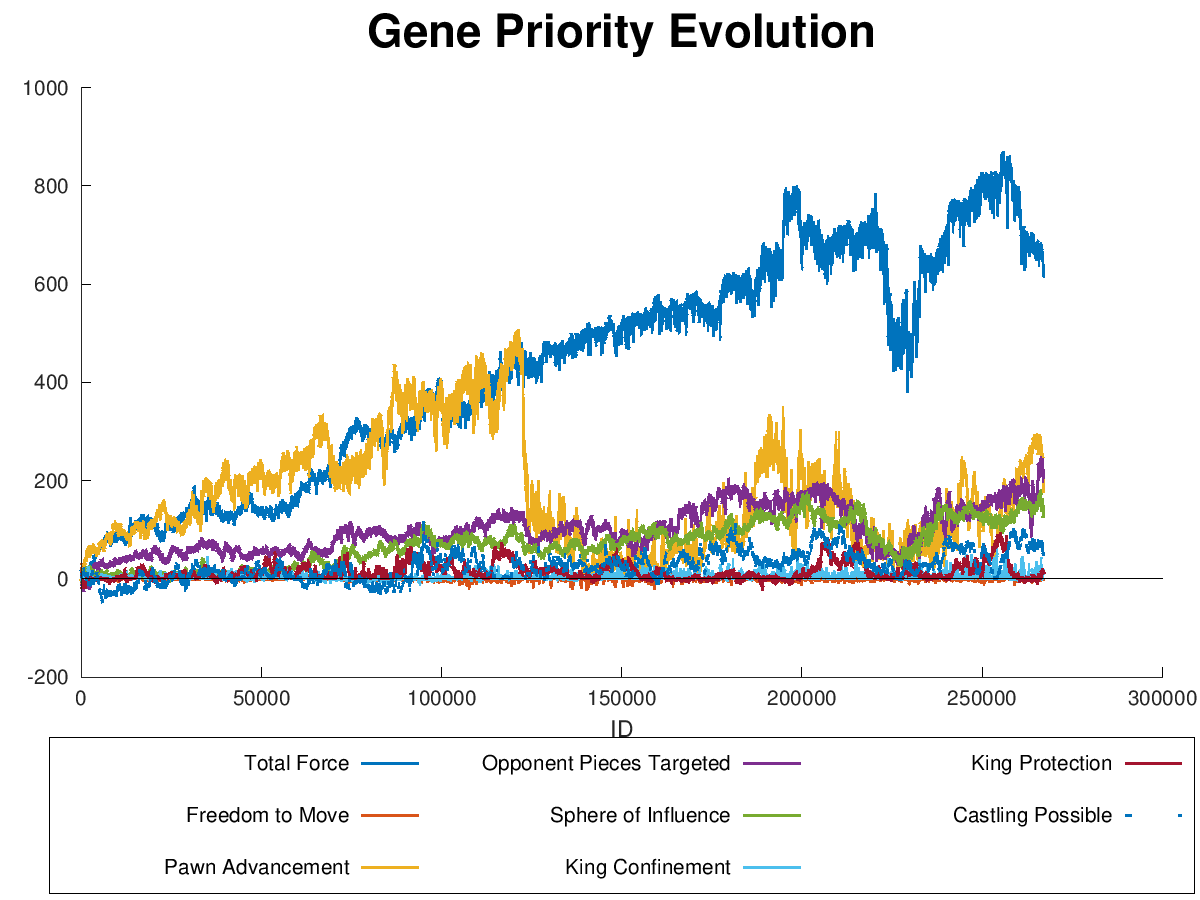
\includegraphics[width=\textwidth]{pawn-advancement-crash}
	\caption{The sudden crash of the Pawn Advancement Gene}
	\label{pawn-crash}
\end{figure}

The only correlation with another gene near that time is in the Piece Strength Gene (see Figure~\ref{piece-value-plot}). The change is small, but in the comparison plot shown in Figure~\ref{pawn-crash}, one can see that the pawn strength has a small jump in value near ID~\#120,000. This is the first time that all of the AIs in the gene pools have strictly positive values for the pawn. Prior to this, the value of a pawn was zero on average. When mutations would push the pawn value higher, it would be weighted too much compared to other pieces, leading to losses and a lower value for the remaining population. It was only when the other pieces reached a large enough value that the pawn value could be properly weighted and sustained. Until this happened, the Pawn Advancement Gene evolved a large value in step with the Total Force Gene since pawns are not actually valueless in real games. Until the Piece Strength Gene transition occurred, the Pawn Advanment Gene served as a proxy for the value of a pawn that was more easily tuned in comparison with the Total Force Gene and Piece Strength Gene. 

This pattern, in which a gene with a lower proper value or priority needs to wait for properly higher-priority genes to evolve high enough priorities before tuning their own priorities, is common and is discussed more the Section~\ref{lower-priority-waits}.

\subsection{The Queen is the most popular piece for promotion.}

Even when the Piece Strength Gene has not been tuned at all, the queen is the overwhelming favorite, followed by the rook, then bishop, and finally the knight. In human games, only the queen and knight are chosen since they have different move patterns. If you need at least a rook or bishop, you might as well take a queen since that piece provides both. Only the knight provides a viable alternative (usually to avoid a stalemate if the queen was chosen).

As an example, the following is a count of all promotions in a gene pool run after more than 300,000 gaes.
\begin{center}
\begin{tabular}{l|r}
	Piece & Promotions \\
\hline
	Bishop & 2232  \\
	Knight  &  1648 \\
	Rook    &  7215 \\
	Queen  & 146664 \\
\end{tabular}
\end{center}


\subsection{Threefold repetition is the most common stalemate.}

Most games with human players end in a draw when neither side can force an advantage. This happens when one side can block a crucial move (e.g., a pawn promotion) and the other side cannot remove this block. Since the blocking player does not have a reason to move, he can just repeat moves to maintain the block. This would lead to threefold repetition if most players did not verbally draw the game beforehand. Since these Genetic AI players don't offer or accept draws, they play out all the repetitions, resulting in what is seen in Figure~\ref{game-ending-plot}.

\subsection{The Look Ahead Gene is a late bloomer.}

The plot in Figure~\ref{game-ending-plot} shows the counts of how games end.
\begin{figure}[htb]
	\centering
	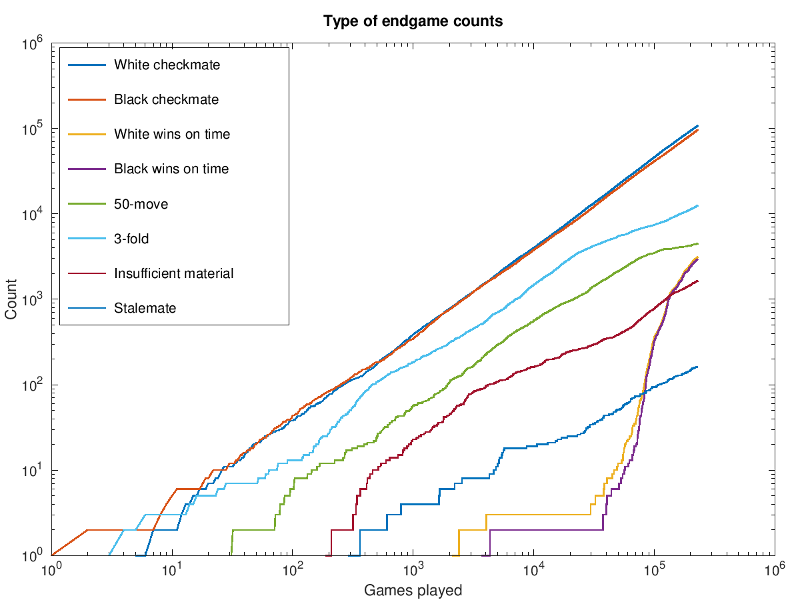
\includegraphics[width=\textwidth]{game-endings-log-plot}
	\caption{A log-log scale of the percentage of games with various endings. Note that the time forfeits don't get going until about 30,000 games in.}
	\label{game-ending-plot}
\end{figure}
It seems that the Look Ahead Gene does not experience significant evolutionary pressure until the board-scoring genes have been tuned to a semi-decent state. My hypothesis is that if the board-scoring function is not able to tell a good position from bad, then looking ahead only increases the risk of losing by time forfeiture with no benefit. However, when the board-scoring genes are in a decent state, the increase in look ahead is very quick. This leads to a rapid increase in the rate of deaths by running out of time, but apparently this is worth the risk as those who are more conservative with their time lose to those who see farther ahead.

\subsection{The Sphere of Influence Gene typically counts legal moves as just as valuable as any other move.}

This was unexpected. I thought that the legal moves would count more since they present a greater threat to the opponent. You cannot capture your opponent's Queen if your own King is in check. Perhaps Genetic\_AIs find this gene more useful as a forward-looking view of the game.

\subsubsection{Late-Breaking News: Update after deleting the Branch Pruning Gene}
The Sphere of Influence Gene now counts legal moves as 50\% more valuable than illegal moves.

\subsection{Genes with properly lower priorities have to wait for higher priority genes to evolve their higher priority before evolving themselves.}
\label{lower-priority-waits}

Some genes are more important than others. The Total Force Gene dominates because it is nearly always more difficult to win when behind in pieces. So, if another gene evolves too high a priority, it hinders game play and will soon be killed off. This means that, because the rate of evolution is the same for all gene priorities, that genes with a lower proper priority\footnote{By proper priority, I mean the as yet unknown relative priority compared with other genes that leads to winning game play. The proper priorities are what this program should be evolving towards.} need to wait for those genes with higher proper priority to evolve a large enough value. Before then, it is too likely for a random mutation to push a lower priority too high and get a gene killed off.

The same goes for the Piece Strength Gene with respect to the value of each type of piece. Note in Figure~\ref{piece-value-plot} that the values rise and fall with each other.

\section{Programmer's Reference}

\subsection{Board}

\subsubsection{ctor()}

Constructs a board in the starting state of a standard chess game.

\subsubsection[ctor(string)]{ctor(const std::string\& fen)}

Construct a board from a string containing a board state in \href{https://en.wikipedia.org/wiki/Forsyth\%E2\%80\%93Edwards\_Notation}{Forsyth-Edwards Notation}.

\subsubsection{legal\_moves()}

Returns a \code{std::vector} of \code{Complete\_Move}s representing all the legal moves of the current board state. Calling this method only generates the list on the first call after a board state change. Every time afterwards it returns a cached copy of the list, so there is no penalty for calling it method multiple times.

\subsubsection{other\_moves()}

Returns a list of moves that are not currently legal but, if they were, would have the moved piece land on a square inside the board. For example, at the beginning of a standard game, the white rook on a1 has no legal moves, as it is blocked in every direction. But, Ra4 would be in the list of other moves, since a4 is on the board and would be legally reachable if the pawn on a2 was not present. Moves to the left or backwards will not be listed, since these moves land outside the board.

\subsubsection[submit\_move]{submit\_move(const Complete\_Move\& move)}
\label{board-submit-move-section}

This method causes the state of the \code{Board} to be changed by enacting the move represented by the argument. Only copies of a move returned from \code{legal\_moves()} will be accepted. Otherwise, an \code{Illegal\_Move\_Exception} will be thrown.



\subsubsection{Important Notes}
\begin{itemize}
\item The \code{Complete\_Move}s returned by the methods \code{Board::get\_complete\_move()} and \code{Board::legal\_moves()} should not be passed around far away from the Board that returned them as there is no guarantee they represent valid moves for a different board or the originating board after it has changed state. A \code{Complete\_Move} generated by one \code{Board} is only valid for another \code{Board} if it is an unmodified copy of the originating \code{Board}.

\item Similarly, a \code{const Piece*} returned by \code{Board::view\_piece\_on\_square()}, is valid for the unmodified Board that returned it. If the \code{submit\_move()} method is called on the originating Board, that piece might be captured, which could result in the \code{Piece*} pointing to deleted data.

\item When calling \code{Board::view\_piece\_on\_square()}, an empty square is represented by a \code{nullptr}.
\end{itemize}

\subsection{Piece}

\subsection{Move}

\subsection{Complete\_Move}

\subsection{Clock}

\subsection{Player}

\subsection{Gene}

\subsection{Genome}



\begin{thebibliography}{9}

\bibitem{evolved-antenna}
G.S. Hornby, A. Globus, D.S. Linden, J.D. Lohn, ``Automated Antenna Design with Evolutionary Algorithms.'' AIAA

\bibitem{evolved-stellarator}
W.H. Miner, Jr., P.M. Valanju, S.P. Hirshman, A. Brooks, N. Pomphrey, ``Use of a genetic algorithm for compact stellarator coil design.'' IAEA Nuclear Fusion, Vol. 41, No. 9. 1185-1195

\bibitem{log-norm-wiki}
\url{https://en.wikipedia.org/wiki/Log-normal\_distribution}

\bibitem{log-norm-chess-se}
\url{https://chess.stackexchange.com/a/4899/5819}

\end{thebibliography}

\end{document}
